\documentclass[12pt]{article}
\usepackage{sbc-template}
\usepackage{graphicx,url}
\usepackage[brazil]{babel}
\usepackage[utf8]{inputenc}
\usepackage{listings}
\usepackage{color}
\usepackage{scalefnt}
\usepackage{soul}
\sloppy

\title{Borboleta and SaguiSaúde - Open Souce Mobile Telehealth for Public Home Healthcare}

\author{Gustavo Luiz Duarte, Rafael Correia, Pedro Leal, Helves Domingues, \\
		Fabio Kon, Rubens Kon, João Eduardo Ferreira}

\address{
        Departamento de Ciência da Computação, Instituto de Matemática e Estatística\\
    Universidade de São Paulo
    \email{\{gduarte, rafaeljpc, pedro.leal, hhdomingues, kon, rkon, jef\}@ime.usp.br}
}

\begin{document}

\maketitle

\begin{abstract}
   	Healthcare Centers play a major role in the Brazilian public healthcare system
	Healthcare Centers play a major role in the Brazilian public healthcare system
	Healthcare Centers play a major role in the Brazilian public healthcare system
	Healthcare Centers play a major role in the Brazilian public healthcare system
	Healthcare Centers play a major role in the Brazilian public healthcare system
	Healthcare Centers play a major role in the Brazilian public healthcare system
\end{abstract}

\section{Introduction}

% cenário e motivação
Healthcare Centers play a major role in the Brazilian public healthcare system as they are responsible for the primary care in their geographic region. Governmental initiatives such as the Family Health Program have produced outstanding results in the improvement of health indexes by focusing on preventive medicine. In these programs, health professionals and specially-trained community agents visit the homes of patients (mostly in low-income, unfavored neighborhoods) to provide health services. However, at the current stage, these actions are carried out with almost no support from Information Technology. All the data is hand-written in forms that are stored in piles of thousands of pieces of paper that are hardly ever used for any significant health action or study.

% hipotese/objetivos
The Borboleta project conducted by the University of São Paulo, Brazil, aims at developing a mobile Open Source Integrated System for management of health information in the context of public healthcare centers and home healthcare service. The hypothesis we want to verify is that automating data collection and processing can improve significantly the quality of the service provided to the population. To achieve that objective, the system we are developing includes a multimedia electronic health record (EHR), which stores patient personal and health data, including treatment history. The mobile EHR improves the quality of the health service, facilitating access to patient health information and guaranteeing that less data is lost due to hand-written records that are not processed. It will also help to identify the evolution of diseases as the health information database is linked to temporal and geographical information.

\section{System architecture}
% abordagem, proposta
The system is composed of two major parts: Borboleta, that runs on smartphones, and SaguiSaúde, that runs on the Healthcare center. During homecare, health professionals visit patients carrying smartphones with Borboleta to store collected information. SaguiSaúde is responsible for centralizing health information of all attended patients and making it easily available for health professionals. SaguiSaúde is used as a support system for all activities regarding patients in the Healthcare center. Developing such a complex system that is easy to use is a challenging effort.


\subsection{Server}
%% Sagui 
SaguiSaúde was developed as a Web system using Ruby on Rails framework and is accessed by health professionals via commodity Web browsers. The system manages patient personal and socioeconomic data, health appointment scheduling and description, drug prescriptions, lab exams, and health professional information. Figure \ref{dataModel} presents the conceptual model of the system.

\begin{figure}[ht]
\centering
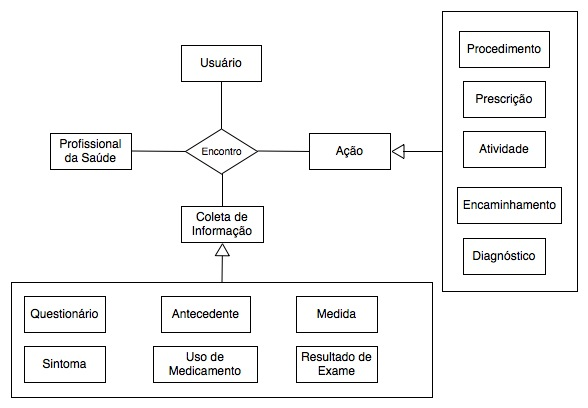
\includegraphics[width=.60\textwidth]{images/ModeloConceitualSagui.jpg}
\caption{Conceptual model}
\label{dataModel}
\end{figure}


This diagram shows clearly the focus of the Healthcare center activities and SaguiSaúde: the Health Appointment. By appointment we mean all occasions in which patient and health professional meet each other, be it in the patient's home due to a routine visit, or be it in the Healthcare center. The requirement elicitation and analysis performed to reach this conceptual model is described in details in \cite{sagui}.

Flexibility in the evolution of the system is mandatory. New features and changes in the existing ones, are frequent. Changes of requirements and new demands from government agencies are common in a Healthcare center. 



Administration

One major concern during the development of a health system is security. SaguiSaúde manages sensitive data, and needs to assure that only permitted users will have access to data. To achieve this, the system has a role based access control module that gives the administrator the ability to manage users and what data each user has access.
% auditoria


SaguiSaúde is composed of 3 main modules: cadastro de pacientes, administration, e encontros.

cadastro de pacientes armazenas dados pessoais e dados socioeconomicos.
o modulo de administraçao gerencia os campos desses formularios, os usuários do sistema, e outros dados como cadastros de exames, ruas, etc.

A motivaçao do desenvolvimento do sagui era automatizar a coleta e armazenamento dos dados de saúde do cseb e facilitar os procedimentos utilizados pelos profissionais de saúde. 

Para antender as necessidades do centro de saude, os desenvolvedores participaram junto com os profissionais de saude na especificacao do sistema. Foi desenvolvido utilizando xp (prototipos).


Um bom modelo de dados se faz necessário pois vamos ter uma porrada de registros. O número de usuários do cseb hoje passa de 170 mil. O modelo de dados do SaguiSaúde é apresentado na figura a seguir.



Health systems use to have complex data models. There is many research in this field, for example the HL7 standard.  


All this data is stored in a PostgreSQL database that is managed by health professionals via a user-friendly Web interface implemented using the Ruby on Rails technology.



- complexidade do modelo (HL7)
- tipos de dados (cadastro de pacientes, exame, agendamento, medicamentos, etc.)
- foco no encontro (histórico)
- necessidade de administração
- flexibilidade na administração dos tipos de dados (tabelas de apoio)
- segurança (audição, usuários)
- tecnologias utilizadas (rails, postgres, ...)





\subsection{Mobile}
%% Borboleta
The Borboleta module \cite{correia08} aim to be a mobile Eletronic Health Record system, which runs on smartphones and PDAs, changing the paper forms that was used before. So the health care providers will gain mobility, because a mobile device is smaller than a bunch of paper forms, and agility, as the system is optimized to not need so much typing on the inputs.

The module carry a subset of the information stored in the central database. This subset is defined based on the homes that will be visited in that particular day, then the data is transfered to the mobile system through the Wi-Fi network at the Healthcare Center. From this step the Borboleta works disconnected from the server module. At the patient home, the health professional has no network access, for this reason we made the mobile modules without a network connection, so they can freely see and update the patient data. At the end of the day, health professionals goes back to the Health Center and synchronize the collected data.

Another aspect that we focus our work is interface of the system. To better fit to the healthcare providers needs the interface must legible and easy to collect. As long as we developed the system under JavaME technology, we could use the default interface toolkit, known as LCDUI, but this toolkit does not have all the requirements to fit our needs, so we look after another interface framework and found the LWUIT, which has a better look and much more interesting component.

\subsection{Synchronizing}
%Sincronização

The synchronizing process is composed of 3 phases: replication, evolution, and reconciliation. In the replication phase, selected records are replicated to mobile device, and, when applicable, data locks are applied. Data locks are meant to avoid data conflicts when a record can be updated in more than one device while replicated. Another approach is to tolerate data conflicts and handling with it during reconciliation, resolving automatically or with human support. In the current state of the system, it is assumed there will be no data conflict. We assure this by replicating records as disjoint sets between mobile devices and reconciling it right after patients visits. The evolution phase is when local updates are applied to the mobile database, during homecare. In the reconciliation phase, updates are propagated from mobile to central database, making collected data globally available in the system. 

During the development of Borboleta and SaguiSaúde we realized that it is unnatural to maintain the same model for the mobile and central databases. Having different, or heterogeneous, data models decouples the development of both systems. However, synchronizing heterogeneous databases implies the addition of another step in the replication and reconciliation phases: data transformation. In [3] we explore in details the motivation and different possible approaches to heterogeneous database synchronization. We've implemented it as a module of SaguiSaúde using Ruby on Rails. It is the only piece of code that is aware of such heterogeneity. It is responsible for transforming data from central to mobile model during replication, and back to central model during reconciliation. To keep this transformation process flexible, the synchronization module is supplied with an external mapping description. Therefore, when one of these models is changed, we just need to change the mapping description, keeping the synchronization code untouched.

Although mobile and central databases have different representations of the same information, they are not independent databases, we must keep the mobile model smaller than the central model in terms of handled information, i.e., every information modeled by the mobile database must be also modeled by the central database to be possible the synchronization. We've implemented the synchronization protocol based on REST (Resource State Transfer) over HTTP, representing data as XML documents. For the transformations descriptions we used XSLT (eXtensible Stylesheet Language for Transformations).



\section{Results}
% Resultados, Estado atual do sistema
The software is developed using a methodology based on Agile Methods in which preliminary versions of the system are tested by real doctors and nurses monthly and several releases are produced each year. Although SaguiSaúde and Borboleta are not yet in production, some of their modules are already usable and tests are being conducted with a 120,000 people database from the University Healthcare center. The system is available as open source software and can be downloaded with a BSD license from http://ccsl.ime.usp.br/borboleta .

\section{Acknowledgment}
The Borboleta project is supported by Microsoft Research-FAPESP Virtual Institute.

\bibliographystyle{sbcbib}
\bibliography{medetel}

\end{document}
